\subsection{Ind-étale maps, exact colimit relations and nil-ideal lifting}\label{algebra-proof-059-ind-uxe9tale-maps-exact-colimit-relations-and-nil-ideal-lifting}

\subsubsection{Source, comparison and coverage}\label{algebra-proof-059-source-comparison-and-coverage}

Source: the Stacks Project authors, algebra.tex at a04446e57ec1fbc252a871afcec7752fb2807b14, SHA-256 FA8BB92E58A4F78A2BD01B3B6A4A87DE0A0D279F5DD90641B574DD5FBFFFA4F3. The complete interval 42761--42958 and its seven received reports were read. The following opening 42959--43060 was also read, without adjudication. No prior canonical correction operation occurs in 42761--42958. Fresh dependency reading: 31885--31990, 39289--39326 and 39507--39538. The previously checked source descent result at 39309--39311 and its editorial treatment are reused, without claiming that its surrounding proof was newly read in this interval.

The four indexed hits from the saved query ``ind etale'' remain unread. The source-reading route retains the seven earlier external readings. Earlier complete proof dependencies are the sections ``Canonical infinitesimal map and nil ideals'' in ALGEBRA\_ETALE\_NOTES\_20260928.md, the diagonal construction in ALGEBRA\_UNRAMIFIED\_NOTES\_20260928.md, ``Uniqueness, colimits and the nilpotence boundary'' in ALGEBRA\_CONORMAL\_THICKENING\_NOTES\_20260928.md, and the complete/nil lifting and local-target sections of ALGEBRA\_HENSELIAN\_NOTES\_20260929.md. The new arguments below receive groups1127,1204,1214,1235,1236. There is no novelty claim. All expanded proofs and strengthened conclusions remain editorial material, separate from the translation.

An R-algebra is called ind-étale here precisely when it is a filtered colimit of étale R-algebras. Rings and maps are commutative and unital; the zero algebra is retained. All diagrams are small. Finite-presentation arguments below refer to actual chosen presentations and every relation.

\subsubsection{The source colimits and their exact comparison maps}\label{algebra-proof-059-the-source-colimits-and-their-exact-comparison-maps}

If E=R{[}x\_1,\ldots,x\_n{]}/(F\_1,\ldots,F\_m) and B is the filtered colimit of B\_i, a map E→B descends by choosing one stage for all n generator images and then a later stage where all m relation errors vanish. Two such maps which agree in B agree at a common later stage: each of the finitely many generator-image differences is eventually zero. For a filtered category rather than a directed set, use the finite-cocone and parallel-arrow equalization axioms at these same finite steps. This proves the exact bijection

\[
\mathop{\rm colim}_i\operatorname{Hom}_R(E,B_i)
\ \longrightarrow\ \operatorname{Hom}_R(E,\mathop{\rm colim}_iB_i).
\]

Keep A=colim\_i A\_i and an arbitrary original map R→R'. The base-change map sends r'⊗a\_i to r'⊗{[}a\_i{]}. Its inverse is the map R'⊗A→colim\_i (R'⊗A\_i) induced by r'↦{[}r'⊗1{]} and {[}a\_i{]}↦{[}1⊗a\_i{]}. Filtered-colimit equalities prove that the second prescription is independent of the representative. The balancing relation over R holds at every stage. The two maps are inverse on every elementary tensor. Each R'⊗A\_i is étale over R', proving 42770--42780 with all original objects retained. Delete only the duplicated words ``so is'' in its conclusion.

For composition R→A→B, write A=colim\_i A\_i with A\_i étale over R, and B=colim\_j B\_j with B\_j étale over A. Given a finitely presented R-algebra P and a map P→B, first descend it to B\_j. Étale descent 39309--39311 provides i and an étale A\_i-algebra B'\emph{j with the specified isomorphism A⊗}(A\_i)B'\emph{j→B\_j. The original map P→B\_j then descends to A}(i')⊗\_(A\_i)B'\emph{j for a later i'. This algebra is étale over R: base change makes it étale over A}(i'), and composition gives the R-map. The displayed factorization is through this exact algebra; it neither asserts B'\_j=B\_j nor changes the given map to B. The finite-presentation factorization criterion 31951--31980 proves B ind-étale over R. At 42807 replace the incomplete initial ``As'' by ``The map'' and its second causal ``as'' by ``since''.

For use in the omitted details, here is the factorization criterion with its maps. Suppose every map P→B from a finitely presented R-algebra factors through an étale R-algebra. Let C\_B have objects (E,u), where E is étale over R and u:E→B; maps are R-maps respecting u. It is essentially small, since finite presentations have a set of possible finite tuples of coefficients and equations. It is nonempty by the factorization of R→B. Two objects map to a third by applying the hypothesis to their tensor product. To equalize two maps E⇉F over B, choose finite algebra generators e\_1,\ldots,e\_n of E and put

\[
D=F/(f(e_1)-g(e_1),\ldots,f(e_n)-g(e_n)).
\]

This is finitely presented over R and maps to B; factor D→B through an étale algebra. This gives the required equalizing arrow from F. Thus C\_B is filtered. Its canonical colimit map to B is surjective: the map R{[}T{]}→B for each b factors through an object. It is injective: if e∈E maps to zero, the finitely presented E/(e) maps to B and factors through another object, making e zero there. The same argument applied to a difference compares any two representatives. This proves the criterion as an isomorphism, with the original receiving maps.

Now retain the source's iterated system A\_i=colim\_(j∈J\_i) A\_(i,j), and A=colim\_i A\_i. A finite presentation P→A first descends to one A\_i and then to an A\_(i,j). The criterion proves that A is ind-étale. It also verifies the source's explicitly given category J. For two objects (i,j),(i',j'), choose a common later i'\,' in I; finite presentation sends both algebras into a common stage of J\_(i'\,`). For parallel arrows from (i,j) to (i',j'), their composites to A\_(i') agree. Their finitely many generator-image differences become zero at a later stage of J\_(i'), which equalizes them. Thus J is filtered. The map colim\_J A\_(i,j)→A sends each element to its original image. Every element of A has such a representative. If two representatives become equal, first compare them at a common A\_k, then at a common stage of J\_k, enlarging that stage for the equality itself. They therefore agree in colim\_J. This proves the claimed isomorphism. The word sequence ``category with objects \ldots{} and morphisms triples'' has two parallel noun phrases; a missing copula is not a defect. The proposed ``and morphisms are triples'' would break that construction.

For a filtered system of actual ring arrows R\_i→A\_i, with limits R,A, the source comparison is

\[
\theta:\mathop{\rm colim}_i(A_i\otimes_{R_i}R)\longrightarrow A,
\qquad [a_i\otimes r]\longmapsto [a_i]r.
\]

Its inverse sends {[}a\_i{]} to {[}a\_i⊗1{]}. For any r∈R, choose its representative r\_j and a common stage k for i,j; the equality a\_i⊗r=(a\_i r\_k)⊗1 holds in A\_k⊗\_(R\_k)R. This proves that the inverse respects the R-action, and that the two compositions are the identity. Base change and the iterated-colimit result apply to the exact rings in θ, proving 42842--42856.

Finally keep the original R-map u:A→B between ind-étale R-algebras, with presentations A=colim\_i A\_i and B=colim\_j B\_j. Form the category T of triples (i,j,t), where t:A\_i→B\_j represents u on that stage. A morphism uses transitions i→i',j→j' and the equality t' a\_(ii')=b\_(jj')t. Each t is étale by 39507--39530. Thus

\[
D_{i,j,t}=A\otimes_{A_i,t}B_j
\]

is étale over A, and it has the specified map a⊗b↦a u\_j(b) to B, where the product uses u:A→B and u\_j:B\_j→B. The category T is filtered. For two triples, choose a common later i', factor A\_(i')→B through some B\_k, and then enlarge k to receive both original B\_j's. The two compatibility equations hold in B; finite generation of the two A\_i's makes them hold at a still later stage. For two parallel arrows, first equalize their underlying index arrows in the filtered indexing categories, and use the same finite equality argument for the resulting factorization maps. Equivalently, for the directed-set presentations used in the source there is at most one such transition between fixed triples.

The map colim\_T D\_(i,j,t)→B is surjective. Every b∈B comes from some B\_j; start with any triple and enlarge its B-index to receive that B\_j. For injectivity, an element of a D\_(i,j,t) is a finite sum Σ a\_l⊗b\_l. Choose a later A\_(i') representing every a\_l, and then a later triple (i',j',t') as above. In that stage this sum is the element 1⊗Σ t'(a\_l)b\_l. If its image in B is zero, enlarge j' once more to kill this exact sum. It is then zero in the displayed colimit. These are the full comparison maps behind 42858--42878; no claim of injectivity of any stage map is used.

\subsubsection{Arbitrary small colimits and the full idempotent relations}\label{algebra-proof-059-arbitrary-small-colimits-and-the-full-idempotent-relations}

The preceding source results admit the following stronger conclusion: the full subcategory of ind-étale R-algebras is closed under every small colimit calculated in R-algebras. Finite diagrams of étale R-algebras have étale colimits. We construct both the original colimit and the maps proving these statements.

First recall the exact diagonal calculation, including its determinant. For an étale R-algebra E with algebra generators z\_1,\ldots,z\_n, put D=E⊗\emph{R E, μ(a⊗b)=ab, and I=ker μ. Its actual generators are δ\_i=z\_i⊗1−1⊗z\_i. The differential identification I/I²=Ω}(E/R)=0 gives I=I². Choose c\_ij∈I with δ\_i=Σ\_j c\_ij δ\_j and retain

\[
e_E=\det(1-C)
 =\sum_{\sigma\in S_n}\operatorname{sgn}(\sigma)
   \prod_{i=1}^n(\delta_{i,\sigma(i)}-c_{i,\sigma(i)}).
\]

The adjugate identity gives e\_E δ\_i=0, hence e\_E I=0. Every nonconstant determinant summand contains an entry of I, so e\_E−1∈I. Thus e\_E²=e\_E and I=(1−e\_E)D. The empty determinant is 1. The idempotent is independent of choices: if e and e' have the same properties, e(1−e')=e'(1−e)=0, whence e=ee'=e'.

For any two R-maps f,g:E→Q, let

\[
\rho:E\otimes_RE\to Q,\quad a\otimes b\mapsto f(a)g(b),
\qquad d_{f,g}=\rho(e_E).
\]

It is an idempotent. The exact ideal generated by all f(x)−g(x) is (1−d\_(f,g))Q: the generators are precisely the images of the diagonal generators, and I=(1−e\_E)D gives both inclusions. Consequently Q/(1−d) and Q\_d represent equality of f and g after a further Q-map. Their inverse comparison maps are q mod(1−d)↦q/1 and q/d\^{}m↦q mod(1−d). The relation d=1 in each ring proves that these prescriptions respect denominators, including d=0 and d=1.

Let B\_• be the given small diagram of ind-étale R-algebras, indexed by a category K. Its actual coproduct in R-algebras is

\[
Q=\bigotimes_{k\in\operatorname{Ob}K,R} B_k.
\]

The empty tensor product is R. A finite tensor product of ind-étale algebras is ind-étale, by the already proved base-change and composition results. Q is the filtered colimit of those tensor products indexed by finite subsets of Ob K. The iterated-colimit result makes Q ind-étale. Write ι\_k:B\_k→Q for the original coproduct maps.

For each arrow v:k→l, choose the given filtered presentation B\_k=colim\_λ E\_(k,λ) by étale R-algebras. Compose each stage map with the two original maps ι\_k and ι\_l B(v), obtaining f\_(v,λ),g\_(v,λ):E\_(k,λ)→Q. Define d\_(v,λ) by the full determinant construction above. The ordinary colimit of B\_• is Q/J, where

\[
J=(\,\iota_k(x)-\iota_l(B(v)(x)):
                    v:k\to l,\ x\in B_k\,).
\]

Every x has a stage representative, and each stage image consists of such x's. The preceding equality of ideals therefore proves

\[
J=\sum_{(v,\lambda)}(1-d_{v,\lambda})Q.
\]

For a finite subset F of these pairs, retain the actual product d\_F=∏\emph{(h∈F)d\_h, with d}∅=1. The associated finite sum of ideals is exactly (1−d\_F)Q. In one direction use, for an ordering F=\{h\_1,\ldots,h\_s\}, the full identity

\[
1-\prod_{a=1}^s d_{h_a}
 =\sum_{a=1}^s\left(\prod_{b<a}d_{h_b}\right)(1-d_{h_a}).
\]

In the other direction, (1−d\_h)d\_F=0 gives 1−d\_h=(1−d\_h)(1−d\_F). Thus the exact quotient presentation is

\[
Q/J\ \cong\ \mathop{\rm colim}_{F\ {m finite}}
     Q/(1-d_F)Q
\ \cong\ \mathop{\rm colim}_{F\ {m finite}} Q_{d_F}.
\]

For F⊆G the transition sends q/d\_F\^{}m to q/1 in Q\_(d\_G), because d\_F d\_G=d\_G. The map to Q/J has the same formula with a quotient class. Conversely Q→colim\_F Q\_(d\_F) kills every generator of J: at the stage containing its pair, the associated d\_h is 1. Hence it factors through Q/J. The two induced maps are inverse on Q and on every displayed denominator. This proves the isomorphisms, not merely a correspondence of points or radicals.

Each Q→Q\_(d\_F) is étale, so composition makes Q\_(d\_F) ind-étale over R. Its filtered colimit is ind-étale. This proves the stated arbitrary-colimit closure. If K is finite and every B\_k is itself étale, take E\_(k,λ)=B\_k with its one stage. Q is then a finite tensor product of étale algebras; there are only finitely many arrows and associated d\_h. The quotient is the single localization Q\_d for their product d, and is étale over R. Empty diagrams give R. Changing the chosen stage presentations gives canonically inverse comparison maps, since both constructions have the same specified colimit maps from every original B\_k; their composites fix those maps and are therefore identities by the colimit universal property.

\subsubsection{Nil ideals and the exact reduction equivalence}\label{algebra-proof-059-nil-ideals-and-the-exact-reduction-equivalence}

Let A=colim\_i A\_i be ind-étale over R and let N be any nil ideal of an R-algebra T. Every map A→T/N lifts uniquely to T. This conclusion does not require finite presentation of A or nilpotence of N.

Here are the full stage and compatibility arguments. For the finite presentation A\_i=R{[}x\_1,\ldots,x\_n{]}/(F\_1,\ldots,F\_m), lift the given coordinate images to t\_1,\ldots,t\_n in T. The errors e\_j=F\_j(t) lie in N. Choose b\_j≥1 with e\_j\^{}(b\_j)=0, and put Q=(e\_1,\ldots,e\_m). Then

\[
Q^{1+\sum_j(b_j-1)}=0,
\]

since every monomial of that total degree contains e\_j to at least its specified exponent. If m=0 use Q=0. The coordinate images give A\_i→T/Q. Its unique lift through the successive square-zero maps T/Q\textsuperscript{(a+1)→T/Q}a exists by formal étaleness. It reduces to the prescribed map to T/N. For two possible lifts, the finitely many generator differences generate a nilpotent ideal by exactly the same exponent formula. They agree modulo that ideal; repeated square-zero uniqueness makes them equal. This proves stagewise existence and uniqueness.

For every transition A\_i→A\_j, composing the lift for j gives a lift of the map for i. Uniqueness identifies it with the lift already constructed for i. The lifts therefore form a compatible cocone and define an actual map A→T. A second such map agrees on every stage and is identical. This also proves naturality in T and in A by comparison on each stage.

This is a precise strengthening of groups1204 and1235 for ind-étale sources. The former's formally étale counterexample R→R/J, where J≠0 is a nil idempotent ideal, remains valid. If R/J were ind-étale over R, the identity into R/J would lift across R→R/J by the preceding result. An R-algebra lift s:R/J→R would satisfy s∘q=id\_R, contradicting q(J)=0 and J≠0. Thus that particular formally étale source is not ind-étale. This proves the exact exclusion; it does not infer that every other formally étale map fails to be ind-étale.

Now let N be a nil ideal of R. Reduction A↦A/NA defines an equivalence between ind-étale R-algebras and ind-étale R/N-algebras. It preserves their given colimit constructions. Base change proves that reduction lands in the latter class. For any ind-étale A and any R-algebra B, the ideal NB is nil: each element is a finite sum of multiples of nilpotent elements and the same multinomial exponent argument kills that finite sum. Thus the unique lifting result gives the exact bijection

\[
\operatorname{Hom}_R(A,B)
 \ \longrightarrow\
\operatorname{Hom}_{R/N}(A/NA,B/NB).
\]

For essential surjectivity, write a given ind-étale R/N-algebra C as colim\_i C\_i with C\_i étale. The equivalence for étale algebras in group1127 gives an étale R-algebra E\_i and a specified isomorphism E\_i/NE\_i→C\_i for every i. Full faithfulness of that equivalence lifts each transition uniquely. The lifted identities are identities and the lifted composites are composites by uniqueness, so these are an actual diagram, not separate unrelated lifts. Put E=colim\_i E\_i. Base change gives the specified isomorphism E/NE→C. The Hom bijection just proved makes any two such lifts uniquely isomorphic over their specified reductions.

Finally the ideal and module data are retained exactly. An ind-étale A is flat over R. Indeed, for an injection U→V of R-modules, an element in the kernel of U⊗A→V⊗A has a representative in U⊗A\_i. Its zero image becomes zero at a later V⊗A\_j, and flatness of A\_j forces that representative to be zero in U⊗A\_j. Therefore the original tensor map is injective. Tensoring 0→N→R→R/N→0 with A gives the full exact sequence

\[
0\longrightarrow N\otimes_R A
 \xrightarrow{\ n\otimes a\mapsto na\ } A
 \longrightarrow A/NA\longrightarrow0.
\]

The image is the actual ideal NA. This is the exact comparison between the retained ideal and its tensor product, with no suppression of a kernel or assumption that N has one exponent.

\subsubsection{Residue maps, local targets and filtered local rings}\label{algebra-proof-059-residue-maps-local-targets-and-filtered-local-rings}

In 42882--42899 contraction notation is read along the given maps, not as an injectivity assertion. Write u:R→S and v\_i:A\_i→A. The primes are p=u\^{}(-1)(m\_S) and q\_i=v\_i\^{}(-1)(q). These equalities are what the conventional intersections R∩m\_S and A\_i∩q mean. Both reports alleging an undefined subring intersection are rejected.

The residue maps in the proof are the actual embeddings κ(q\_i)→κ(q) followed by the given τ:κ(q)→κ(m\_S). For a fraction a/b with b outside q\_i, its image is v\_i(a)/v\_i(b); the denominator is nonzero because q\_i is the contraction. Apply the finite-stage henselian-target lemma to obtain f\_i:A\_i→S. For each transition, its composite with f\_j has the same contracted prime and the same residue-field map, so the finite-stage uniqueness proves compatibility. The induced f:A→S has f\^{}(-1)(m\_S)=q: on a representative a\_i membership on either side is membership in q\_i. Its residue-field map sends a/b to the quotient of the residues of f(a),f(b), and equals τ by the stage formula. A second eligible map agrees at every stage and is equal to f.~Replace the shorthand ``f mod q=τ'' by the explicitly typed condition that f induces τ on residue fields. The fraction extension is unique; the source theorem is not false because of that shorthand.

For the two henselian local algebras S,S' with the prescribed common residue field K, apply this lifting result to produce f:S→S' and g:S'→S inducing id\_K. Both composites and the respective identity maps induce id\_K; uniqueness makes gf=id\_S and fg=id\_(S'). This proves the exact isomorphism in 42901--42919.

The local-target consequence of group1236 extends to every ind-étale algebra. Let R be strictly henselian and R→S any local map to a local ring. Then for every ind-étale R-algebra A the map

\[
\operatorname{Hom}_R(A,R)\longrightarrow\operatorname{Hom}_R(A,S)
\]

is bijective. Write A=colim\_i A\_i with A\_i étale. For each i, the finite-stage argument decomposes A\_i into copies of R and a factor of empty closed fibre. A map to S selects exactly one copy; the empty-fibre factor cannot map to κ(S), because its base change to that nonzero field is zero. Thus its map to S comes from a unique map to R. For a given f:A→S, apply this to each f\_i, obtaining g\_i:A\_i→R. For a transition, g\_j composed with it and g\_i have the same composite to S; the finite-stage bijection makes them equal. Their colimit map g satisfies u∘g=f.~Uniqueness follows on the same stages. No nonemptiness of these Hom sets is assumed. R=k with k algebraically closed of characteristic zero and S=k{[}t{]}\_(t) again gives a nonhenselian target: a square in k(t) has even order at t+1, so the simple residue root of X²−(1+t) cannot lift in S.

For completeness, the source's last local-colimit assertion keeps its original local transitions. For a filtered diagram of nonzero local rings R\_i, the residue-field transitions are embeddings. Their filtered colimit κ is a field and every κ\_i→κ is injective: an element that becomes zero does so at a stage, where a field embedding is injective. The map R=colim R\_i→κ is surjective, and its kernel is the ideal represented by the m\_i. If a class x∈R has nonzero residue, its representative in some R\_i has nonzero residue and hence is a unit there; its inverse maps to an inverse in R. Elements of the kernel cannot be units since κ is a nonzero field. Thus R is local with exactly this maximal ideal and residue field, even when the ring transitions are not injective.

If every R\_i is henselian, take the original monic polynomial f over R and simple residue root a\_0∈κ. Choose one stage for all its finitely many coefficients, keeping the leading coefficient equal to 1, and for a\_0. The root and nonzero derivative conditions hold at that common stage because its residue field embeds in κ. Henselianity supplies the required root there, and its image is the required root of the original f.~If every κ\_i is separably closed, a monic separable polynomial over κ descends together with the finitely many coefficients of a Bezout identity for it and its derivative. At that common stage it is separable, hence splits into linear factors in κ\_i. Passing those exact factors to κ shows that κ is separably closed. This proves the strictly henselian assertion as well.

\subsubsection{Diagram of the proved maps}\label{algebra-proof-059-diagram-of-the-proved-maps}

\begin{figure}
\centering
\pandocbounded{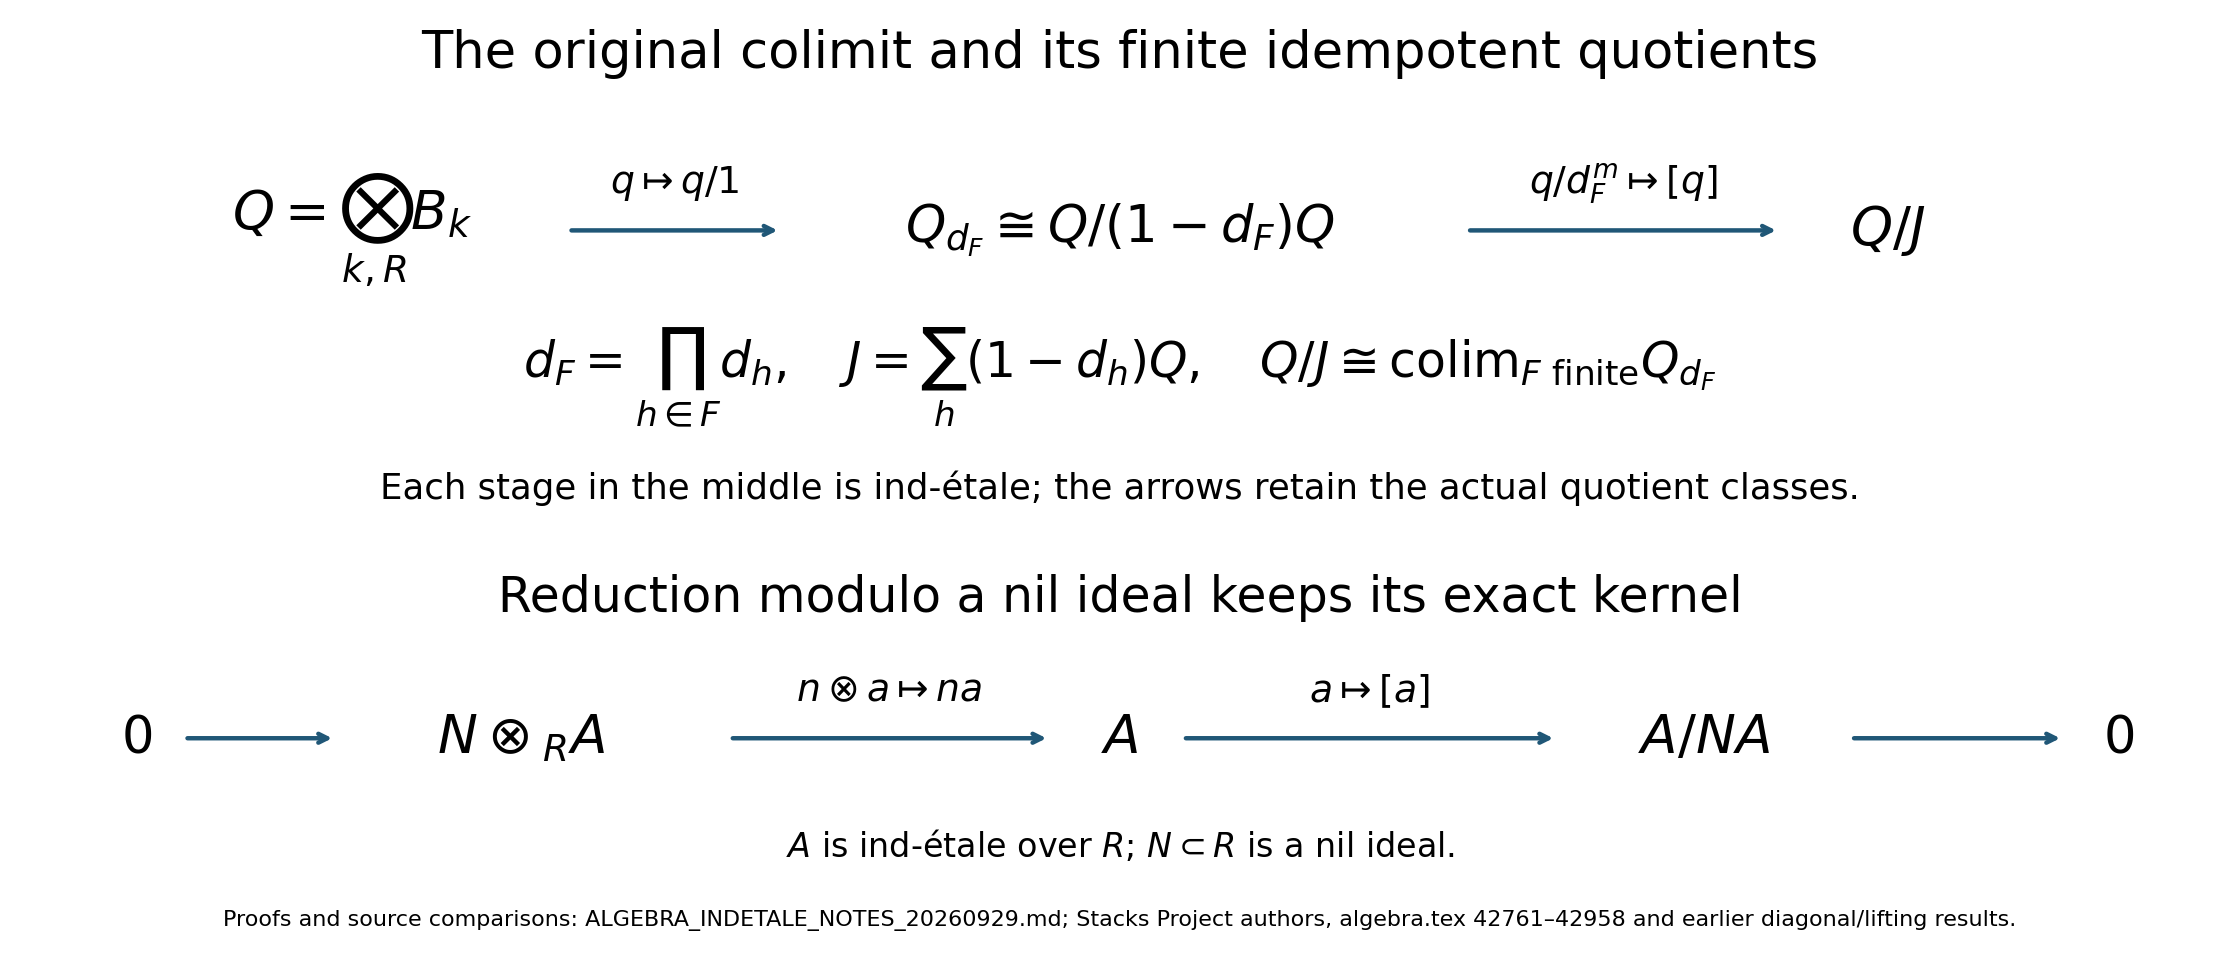
\includegraphics[keepaspectratio,alt={Exact colimit quotients and the nil-ideal sequence}]{INDETALE_COLIMIT_MAPS_20260929.png}}
\caption{Exact colimit quotients and the nil-ideal sequence}
\end{figure}

The top row is the actual coproduct Q, the finite idempotent localizations and their colimit Q/J from the arbitrary-colimit proof. The isomorphism in the middle uses the explicit mutually inverse maps proved there. The bottom row is the exact flat sequence for an ind-étale A and a nil ideal N of R. Both rows retain their original quotient and ideal data. Full proof locators are the two preceding colimit and nil-ideal sections; their human-source comparisons are with the Stacks Project authors at the authority locators listed above. Reproducible source: draw\_indetale\_colimit\_20260929.py; vector edition: INDETALE\_COLIMIT\_MAPS\_20260929.svg. The PNG was inspected for legibility, all arrow directions and mathematical labels.

\subsubsection{Findings and propagation}\label{algebra-proof-059-findings-and-propagation}

Seven reports give two copyedits, one typed residue-map clarification, and two rejected groups: the parallel noun phrases and the two contraction notations are not source defects. The source proofs of filtered closure and henselian lifting remain identifiable.

Three separate consequence groups receive earlier proofs. The first uses group1214's exact diagonal idempotent to prove all-small- colimit closure with the original tensor product, full difference ideal and every finite idempotent product. The second receives groups1127,1204,1235 and proves arbitrary nil-ideal lifting and reduction equivalence for ind-étale algebras, with the exact flat ideal sequence and the non-ind-étale counterexample boundary. The third receives group1236 and proves the Hom-set bijection for arbitrary local targets and all ind-étale sources. These are not substitutions for the original translated arguments. Broader combined-result synthesis and any paper remain after core work.
